\chapter{Processus BPMN d'orchestration}\label{chap:bpmn}

\section{Vue d'ensemble}

Le processus « Candidature » (version 1.0) est modélisé en BPMN~2.0 et exécuté par Bonita Community 2025.2. Il est déclenché à chaque dépôt et couvre les neuf étapes de l'énoncé, de la réception de la candidature à la mise à jour du suivi des stages.

Le diagramme comprend un bassin, trois couloirs (Étudiant, Système, Entreprise), dix-huit tâches de service, une tâche humaine, quatre passerelles exclusives, un minuteur de relance, quatre événements de fin et un sous-processus événementiel de gestion des erreurs. Son fichier BPMN (\code{bpmn/processus-candidature.bpmn}) est le même que celui qu'affiche le portail : les identifiants des nœuds sont les noms d'étapes que S4 enregistre dans son journal, ce qui permet de colorer le diagramme au fur et à mesure du traitement (chapitre~\ref{chap:interface}).

\begin{sidewaysfigure}
\centering
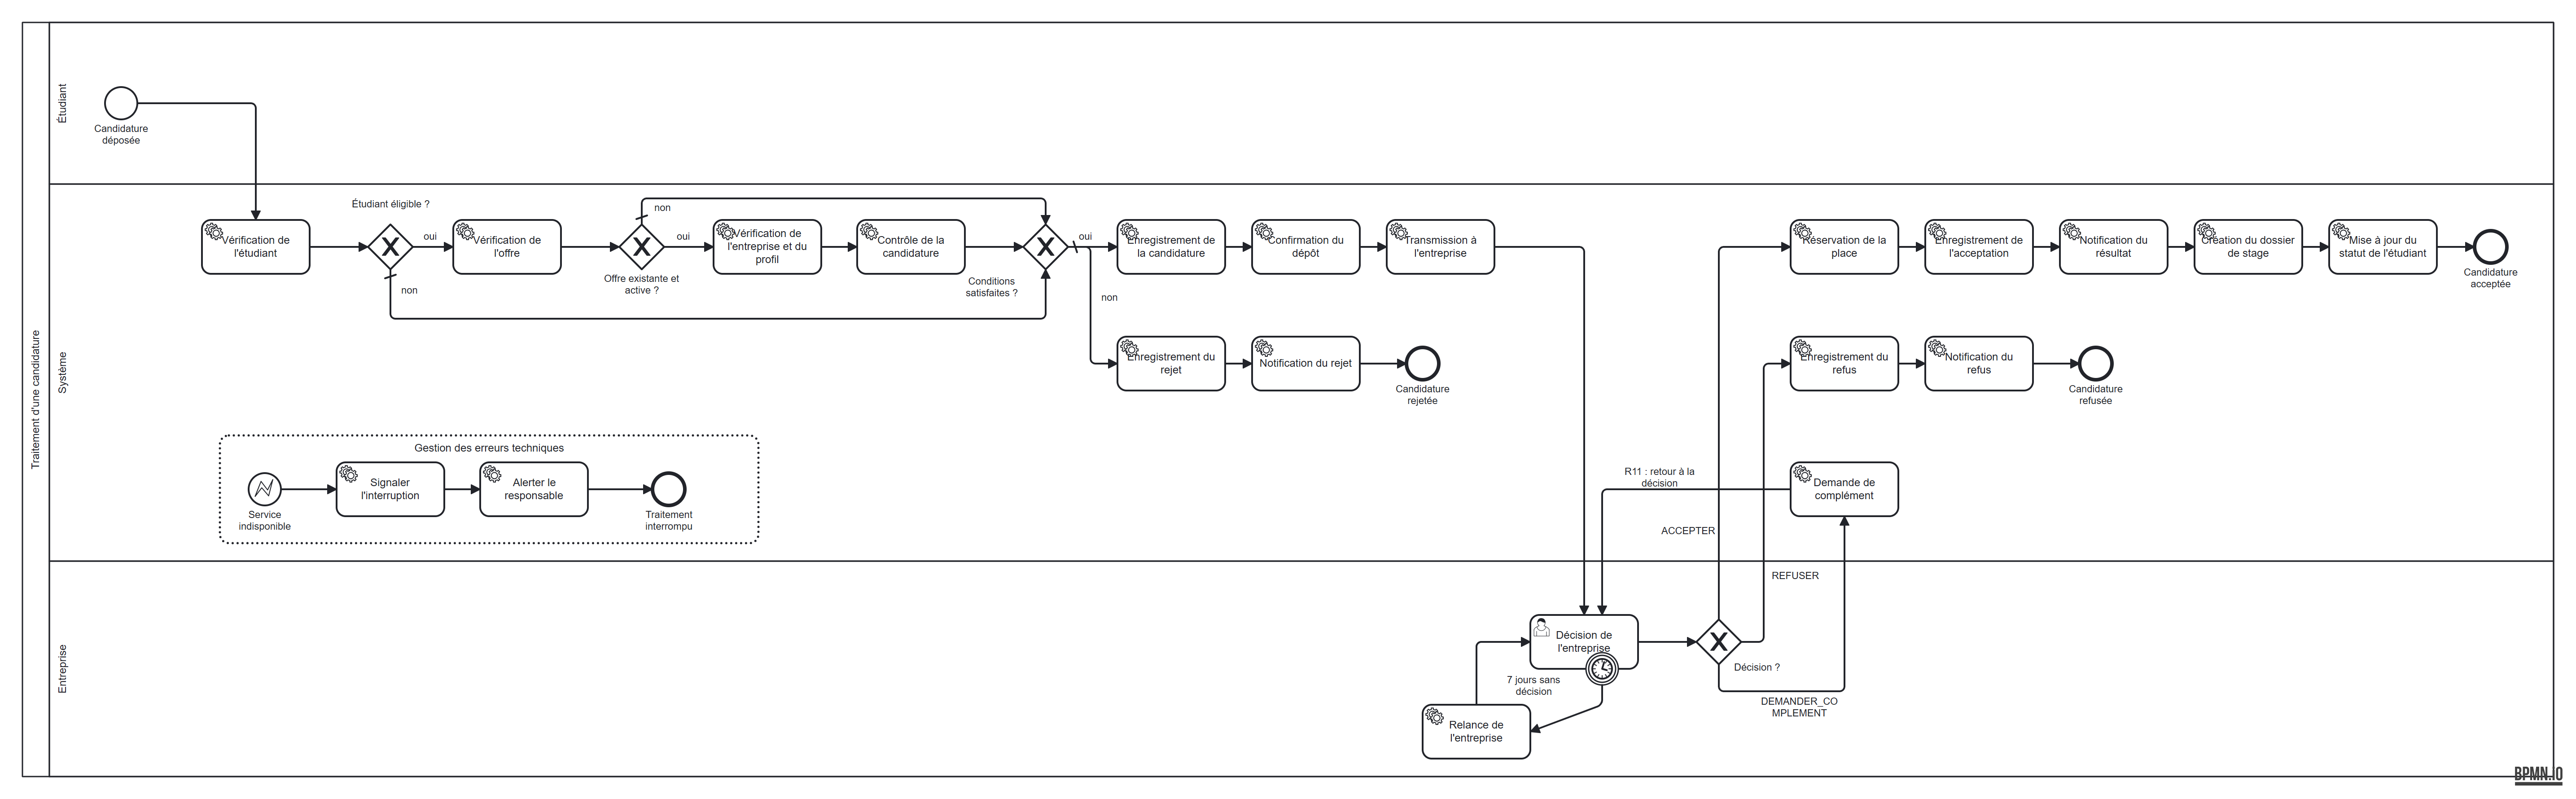
\includegraphics[width=\linewidth]{bpmn-processus.png}
\caption{Processus « Candidature » : diagramme BPMN (rendu par bpmn-js depuis \code{processus-candidature.bpmn})}\label{fig:bpmn-export}
\end{sidewaysfigure}

Le processus existe sous deux formes, qui partagent les mêmes tâches, passerelles et noms :
\begin{itemize}
  \item \textbf{le modèle} (figure~\ref{fig:bpmn-export}) : fichier BPMN à importer dans Bonita Studio, avec des connecteurs SOAP et REST et le sous-processus d'erreur ; sa construction est décrite pas à pas dans \code{docs/bonita/GUIDE\_BONITA.md} ;
  \item \textbf{la version déployée} : construite par programme avec l'API du moteur Bonita (\code{docs/bonita/deploiement}), empaquetée en archive \code{bpmn/Candidature--1.0.bar} et déployée par l'API REST de Bonita (\code{scripts\textbackslash deployer-bonita.ps1}). Elle utilise le \emph{mode secours} du guide : chaque tâche de service est une opération Groovy qui appelle elle-même les services, sans connecteur. Les connecteurs SOAP et REST ne sont en effet pas fournis avec Bonita Community 2025.2 ; ils s'ajoutent depuis la Marketplace.
\end{itemize}
C'est la version déployée qui a été vérifiée de bout en bout face au vrai Bonita (section~\ref{sec:bpmn-verification}).

\begin{figure}[H]
\centering
{\setlength{\fboxsep}{0pt}\color{filet}\fbox{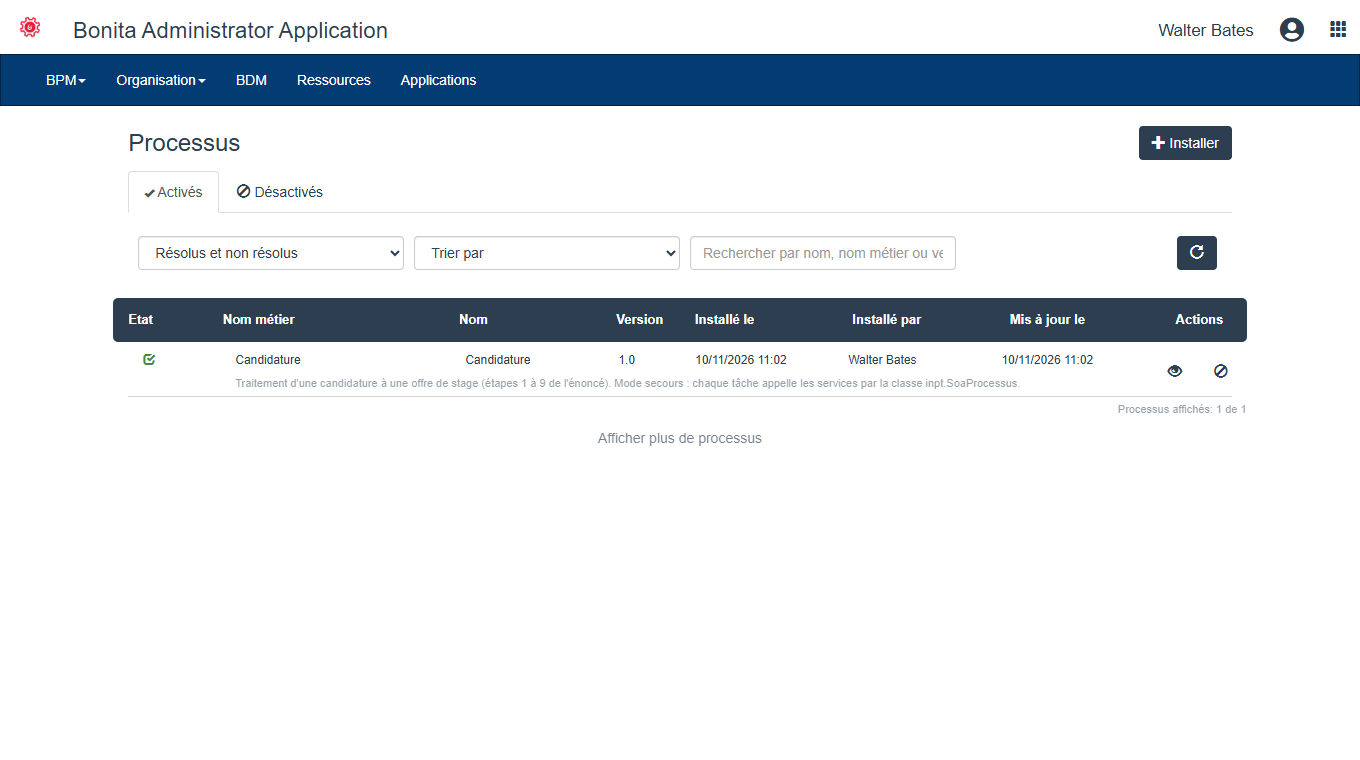
\includegraphics[width=0.9\linewidth]{bonita-processus.png}}}
\caption{Le processus « Candidature » 1.0 déployé et activé dans Bonita (application d'administration)}\label{fig:bonita-processus}
\end{figure}

\section{Déclenchement et données du processus}

S4 démarre un cas par l'API REST de Bonita : connexion (\code{/loginservice}, jeton \code{X-Bonita-API-Token}), recherche du processus par nom et version, puis instanciation avec le contrat suivant.

\begin{table}[H]
\centering\small
\begin{tabularx}{\linewidth}{@{}l l>{\raggedright\arraybackslash}X@{}}
\toprule
\textbf{Entrée du contrat} & \textbf{Type} & \textbf{Rôle} \\ \midrule
\code{soumissionId} & LONG & Soumission créée par S4 ; permet au processus d'écrire dans le bon dossier (journal, rejet, enregistrement). \\
\code{etudiantId} & LONG & Étudiant qui candidate. \\
\code{offreId} & LONG & Offre visée. \\
\code{lettreMotivation} & TEXT & Lettre transmise à l'entreprise. \\
\bottomrule
\end{tabularx}
\caption{Contrat d'instanciation du processus}\label{tab:contrat-bonita}
\end{table}

Le processus n'a qu'une variable, \code{dossier} (une table associative), initialisée à partir du contrat et complétée par chaque tâche (résultat des vérifications, règle violée, identifiant de la candidature, décision…). Avec une seule variable, chaque tâche n'a qu'une opération, et la logique d'appel et de lecture des réponses est regroupée dans une classe Groovy, \code{inpt.SoaProcessus}, livrée dans l'archive du processus et testée hors de Bonita.

\section{Étapes du processus}

\begin{longtable}{@{}>{\raggedright\arraybackslash}p{0.05\linewidth}>{\raggedright\arraybackslash}p{0.27\linewidth}>{\raggedright\arraybackslash}p{0.40\linewidth}>{\raggedright\arraybackslash}p{0.20\linewidth}@{}}
\caption{Tâches du processus et services appelés}\label{tab:taches-bpmn}\\
\toprule \textbf{Étape} & \textbf{Élément BPMN} & \textbf{Appels} & \textbf{Règles} \\ \midrule
\endfirsthead
\toprule \textbf{Étape} & \textbf{Élément BPMN} & \textbf{Appels} & \textbf{Règles} \\ \midrule
\endhead
\bottomrule
\endlastfoot
1 & Candidature déposée (début) & déclenché par S4 à la réception & – \\
2 & Vérification de l'étudiant & SOAP S1 \code{verifierEtudiant} & R1 \\
3 & Vérification de l'offre & SOAP S3 \code{verifierDisponibilite} & R2 (offre) \\
3 & Vérification de l'entreprise et du profil & SOAP S3 \code{consulterOffre}, S2 \code{verifierEntreprise}, S3 \code{verifierCompatibilite} & R2 (entreprise), R7 \\
4 & Contrôle de la candidature & REST S4 \code{verification-doublon}, compte des actives ; date et places d'après S3 & R3 à R6 \\
5 & Passerelle « Conditions satisfaites ? » & – & – \\
5 & Enregistrement de la candidature & REST S4 \code{POST /candidatures} & R5, R6 (garanties) \\
5 & Enregistrement du rejet, Notification du rejet & REST S4 \code{POST /soumissions/\{id\}/rejet}, S5 notification & – \\
6 & Confirmation du dépôt, Transmission à l'entreprise & REST S5 (deux notifications) & – \\
7 & Décision de l'entreprise (tâche humaine) & contrat \{\code{decision}, \code{commentaire}\} & R9 \\
8 & Notification du résultat / du refus & REST S5 & – \\
9 & Réservation de la place & SOAP S3 \code{decrementerPlaces} & R10 \\
9 & Enregistrement de l'acceptation / du refus & REST S4 \code{PATCH /candidatures/\{id\}/statut} & R9 \\
9 & Création du dossier de stage & REST S6 \code{POST /stages} & R10 \\
9 & Mise à jour du statut de l'étudiant & SOAP S1 \code{changerStatutEtudiant} & R10 \\
– & Demande de complément & REST S5, puis retour à la décision & R11 \\
– & Relance de l'entreprise (minuteur de 7 jours) & REST S5 & – \\
\end{longtable}

Chaque tâche inscrit son étape dans le journal de S4 (\code{POST /soumissions/\{id\}/etapes}) : le portail suit ainsi le cas Bonita en direct.

\section{Passerelles de décision}

Les conditions sont des expressions Groovy sur la variable \code{dossier}. Chaque passerelle a un flux par défaut, emprunté si aucune condition n'est vraie : le processus ne peut jamais rester bloqué sur une passerelle.

\begin{table}[H]
\centering\small
\begin{tabularx}{\linewidth}{@{}l l>{\raggedright\arraybackslash}X@{}}
\toprule
\textbf{Passerelle} & \textbf{Flux} & \textbf{Condition} \\ \midrule
Étudiant éligible ? & oui & \code{dossier.etudiantEligible == true} \\
 & non (défaut) & vers la passerelle de décision, qui rejettera (R1) \\
Offre existante et active ? & oui & \code{SoaProcessus.offreValable(dossier)} \\
 & non (défaut) & vers la passerelle de décision (R2) \\
Conditions satisfaites ? & oui & \code{SoaProcessus.conditionsSatisfaites(dossier)} \\
 & non (défaut) & enregistrement du rejet, notification, fin « Candidature rejetée » \\
Décision ? & ACCEPTER & \code{SoaProcessus.decisionEst(dossier, 'ACCEPTER')} \\
 & REFUSER & \code{SoaProcessus.decisionEst(dossier, 'REFUSER')} \\
 & DEMANDER\_COMPLEMENT & \code{SoaProcessus.decisionEst(dossier, 'DEMANDER\_COMPLEMENT')} \\
\bottomrule
\end{tabularx}
\caption{Conditions des passerelles}\label{tab:passerelles}
\end{table}

Les deux passerelles intermédiaires (« Étudiant éligible ? », « Offre existante et active ? ») ne figurent pas dans l'énoncé. Sans elles, un étudiant ou une offre inexistants feraient échouer l'appel suivant (une offre inconnue n'a pas d'entreprise à vérifier) et le cas partirait en erreur technique, alors qu'il s'agit d'un rejet métier ordinaire. Elles court-circuitent les vérifications devenues inutiles et mènent directement à la passerelle de décision de l'étape~5, qui reste le seul point de rejet.

\section{Tâche humaine et boucle de complément}

« Décision de l'entreprise » est une tâche humaine du couloir Entreprise. Son contrat attend une \code{decision} (ACCEPTER, REFUSER ou DEMANDER\_COMPLEMENT, contrainte vérifiée par Bonita) et un \code{commentaire}. L'entreprise décide depuis le portail du projet : S4 vérifie d'abord la règle R10 (une place est-elle encore disponible ?), puis recherche la tâche du cas, se l'assigne et l'exécute par l'API de Bonita.

La demande de complément (R11) passe par la tâche « Demande de complément », qui notifie l'étudiant, puis revient à la décision. Un minuteur de sept jours, en bordure de la tâche humaine, déclenche « Relance de l'entreprise » si aucune décision n'est prise ; la tâche de décision est ensuite recréée. La figure~\ref{fig:bonita-tache} montre un cas en attente : la tâche humaine et son minuteur sont actifs.

\begin{figure}[H]
\centering
{\setlength{\fboxsep}{0pt}\color{filet}\fbox{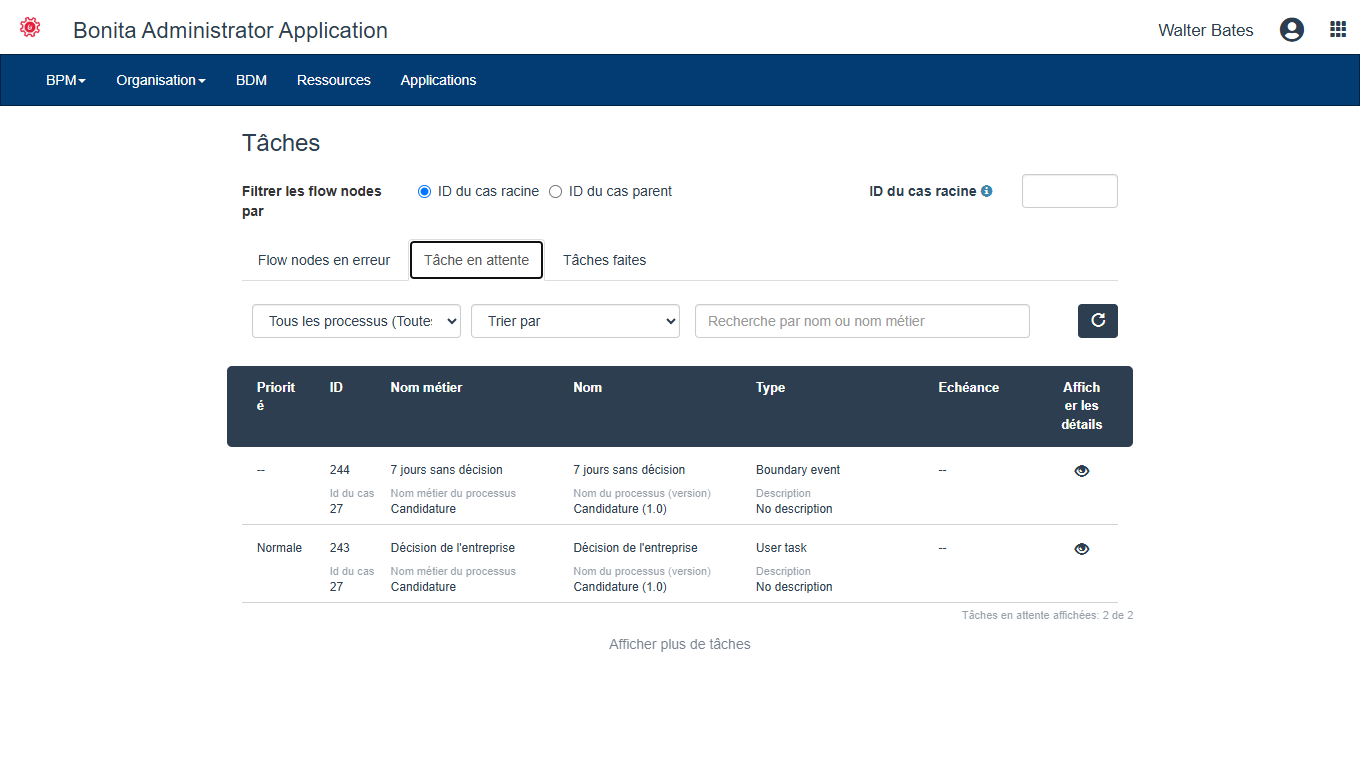
\includegraphics[width=0.9\linewidth]{bonita-tache-decision.png}}}
\caption{Dans Bonita : la tâche « Décision de l'entreprise » en attente, avec son minuteur de relance}\label{fig:bonita-tache}
\end{figure}

\section{Gestion des erreurs et des indisponibilités}

\subsection{Dans le modèle}
Chaque connecteur est configuré pour lever l'erreur BPMN \code{SERVICE\_INDISPONIBLE} s'il échoue (délai dépassé, réponse 5xx, faute \code{ServiceIndisponibleFault}). Un unique sous-processus événementiel, « Gestion des erreurs techniques », intercepte cette erreur où qu'elle survienne : « Signaler l'interruption » (S4 passe la soumission en \statut{ERREUR}, avec la dernière étape réussie), « Alerter le responsable » (courriel \code{ALERTE\_RESPONSABLE}), puis fin « Traitement interrompu ». Un seul sous-processus plutôt qu'un événement de bordure par tâche garde le diagramme lisible et garantit un traitement identique quelle que soit l'étape interrompue.

\subsection{Dans la version déployée}
Sans connecteur, une panne ne peut pas lever d'erreur BPMN : c'est la classe Groovy qui fait le même traitement. Quand un service ne répond pas, la méthode de la tâche signale l'interruption à S4 (soumission en \statut{ERREUR}), envoie l'alerte au responsable, puis échoue : la tâche apparaît « en erreur » dans Bonita (figure~\ref{fig:bonita-erreur}), où un administrateur peut la rejouer une fois le service rétabli. Côté portail, l'étudiant voit « Traitement interrompu » ; aucune candidature à moitié enregistrée ne subsiste.

\begin{figure}[H]
\centering
{\setlength{\fboxsep}{0pt}\color{filet}\fbox{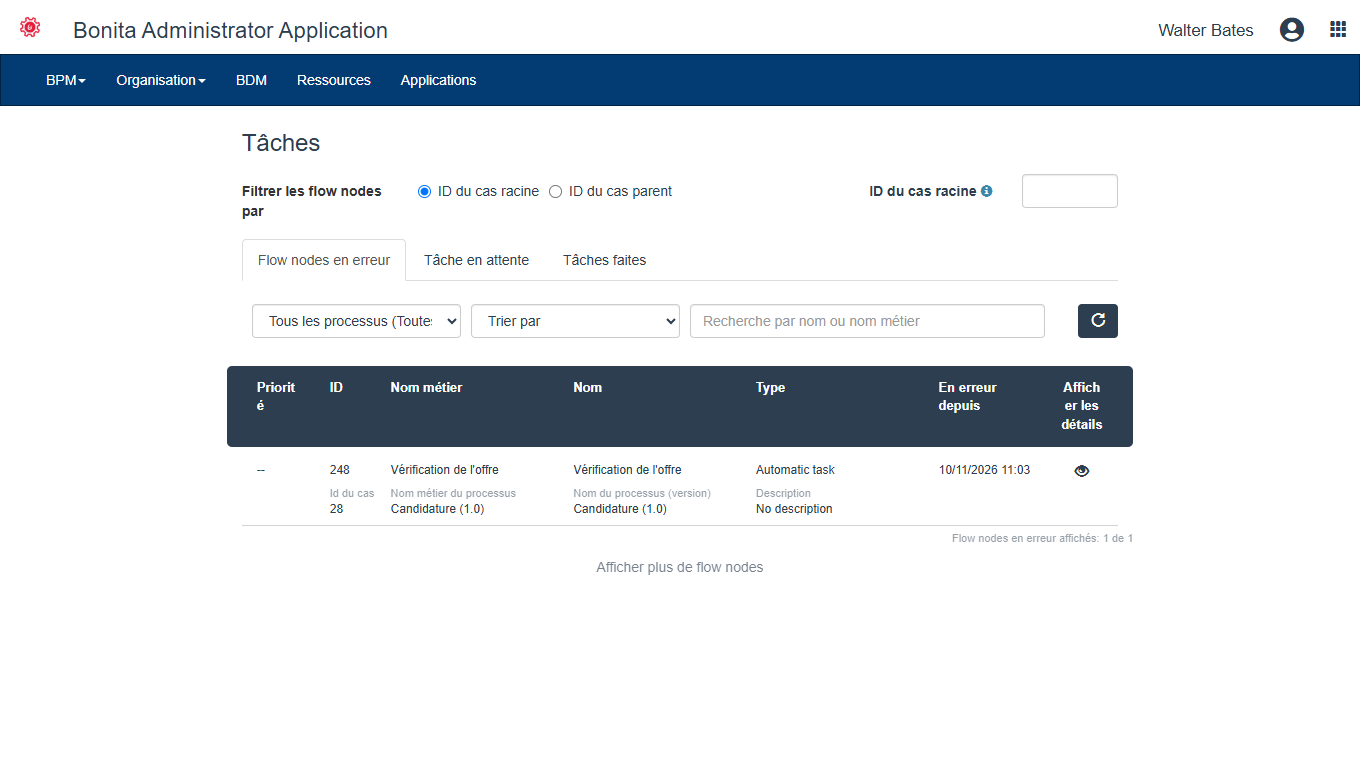
\includegraphics[width=0.9\linewidth]{bonita-taches.png}}}
\caption{Dans Bonita : la tâche « Vérification de l'offre » en erreur pendant une panne de S3}\label{fig:bonita-erreur}
\end{figure}

\section{Connecteurs du modèle}

\subsection{Connecteurs SOAP}
Dans le modèle, les tâches qui appellent S1, S2 ou S3 utilisent le connecteur Web Service (SOAP~1.1) de Bonita. L'enveloppe est produite par la classe Groovy (par exemple \code{SoaProcessus.enveloppeVerifierEtudiant(dossier)}) et contient l'en-tête WS-Security du compte \code{bonita} ainsi que l'identifiant de corrélation du cas. La sortie \code{responseDocumentBody} est lue par la méthode \code{apres…} correspondante, qui met à jour \code{dossier} et inscrit l'étape dans le journal de S4.

\subsection{Connecteurs REST}
Les tâches qui appellent S4, S5 ou S6 utilisent le connecteur REST, avec les en-têtes \code{X-API-Key} (clé du client \code{bonita}), \code{X-Correlation-Id} et \code{Content-Type: application/json}. Les URL et les corps sont, eux aussi, fournis par la classe Groovy. Pour les deux changements de statut (\code{PATCH}), un connecteur qui ne propose pas ce verbe peut envoyer \code{POST} avec l'en-tête \code{X-HTTP-Method-Override: PATCH}, accepté par les services.

\subsection{Mode secours}
En mode secours, la version déployée, chaque tâche est réduite à une seule opération Groovy qui fait l'appel elle-même (par exemple \code{SoaProcessus.verifierEtudiant(dossier)}), avec les mêmes enveloppes SOAP, en-têtes de sécurité et corrélation que les connecteurs. Le comportement métier est identique.

\section{Exécution et vérification}\label{sec:bpmn-verification}

Le processus est vérifié à trois niveaux :
\begin{itemize}
  \item le fichier BPMN est relu sans avertissement par bpmn-moddle, l'analyseur de bpmn-js ;
  \item une simulation (\code{tests/bonita/SimulationBonita.groovy}) répond à l'API REST de Bonita et déroule le graphe tâche par tâche avec la classe livrée, avec connecteurs comme en mode secours ;
  \item surtout, le test de bout en bout a été joué face au \textbf{vrai Bonita Community 2025.2}, processus déployé : les 59 vérifications des scénarios et les 6 de la panne de S3 ont réussi, chaque candidature passant par un cas Bonita.
\end{itemize}

\begin{figure}[H]
\centering
{\setlength{\fboxsep}{0pt}\color{filet}\fbox{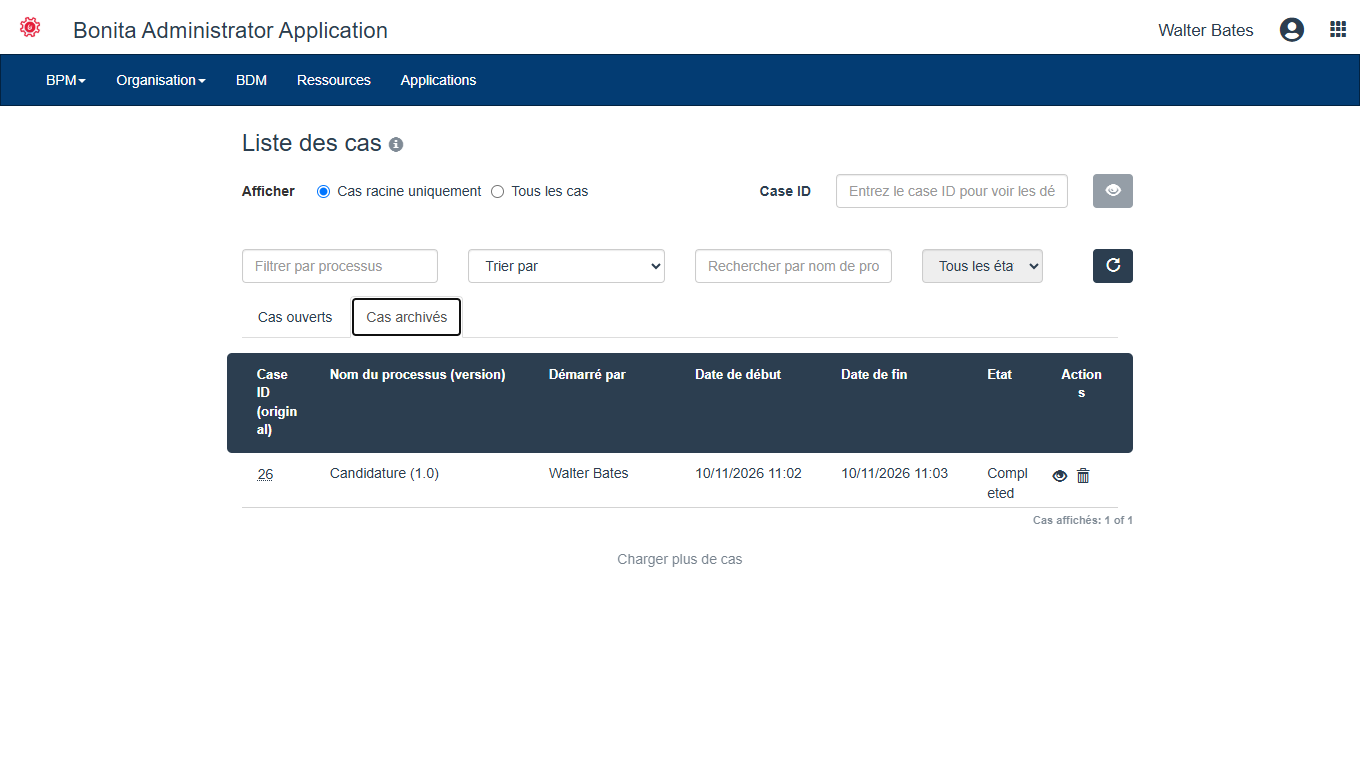
\includegraphics[width=0.9\linewidth]{bonita-cas-archives.png}}}
\caption{Dans Bonita : le cas d'une candidature acceptée, terminé et archivé}\label{fig:bonita-termine}
\end{figure}

Les captures Bonita de ce chapitre sont produites par \code{scripts\textbackslash captures-bonita.ps1}, qui redéploie le processus, joue trois cas réels (acceptation, attente de décision, panne de S3) et capture l'application d'administration de Bonita.
